\documentclass[english,floatsintext,man]{apa6}

\usepackage{amssymb,amsmath}
\usepackage{ifxetex,ifluatex}
\usepackage{fixltx2e} % provides \textsubscript
\ifnum 0\ifxetex 1\fi\ifluatex 1\fi=0 % if pdftex
  \usepackage[T1]{fontenc}
  \usepackage[utf8]{inputenc}
\else % if luatex or xelatex
  \ifxetex
    \usepackage{mathspec}
    \usepackage{xltxtra,xunicode}
  \else
    \usepackage{fontspec}
  \fi
  \defaultfontfeatures{Mapping=tex-text,Scale=MatchLowercase}
  \newcommand{\euro}{€}
\fi
% use upquote if available, for straight quotes in verbatim environments
\IfFileExists{upquote.sty}{\usepackage{upquote}}{}
% use microtype if available
\IfFileExists{microtype.sty}{\usepackage{microtype}}{}

% Table formatting
\usepackage{longtable, booktabs}
\usepackage{lscape}
% \usepackage[counterclockwise]{rotating}   % Landscape page setup for large tables
\usepackage{multirow}		% Table styling
\usepackage{tabularx}		% Control Column width
\usepackage[flushleft]{threeparttable}	% Allows for three part tables with a specified notes section
\usepackage{threeparttablex}            % Lets threeparttable work with longtable

% Create new environments so endfloat can handle them
% \newenvironment{ltable}
%   {\begin{landscape}\begin{center}\begin{threeparttable}}
%   {\end{threeparttable}\end{center}\end{landscape}}

\newenvironment{lltable}
  {\begin{landscape}\begin{center}\begin{ThreePartTable}}
  {\end{ThreePartTable}\end{center}\end{landscape}}




% The following enables adjusting longtable caption width to table width
% Solution found at http://golatex.de/longtable-mit-caption-so-breit-wie-die-tabelle-t15767.html
\makeatletter
\newcommand\LastLTentrywidth{1em}
\newlength\longtablewidth
\setlength{\longtablewidth}{1in}
\newcommand\getlongtablewidth{%
 \begingroup
  \ifcsname LT@\roman{LT@tables}\endcsname
  \global\longtablewidth=0pt
  \renewcommand\LT@entry[2]{\global\advance\longtablewidth by ##2\relax\gdef\LastLTentrywidth{##2}}%
  \@nameuse{LT@\roman{LT@tables}}%
  \fi
\endgroup}


  \usepackage{graphicx}
  \makeatletter
  \def\maxwidth{\ifdim\Gin@nat@width>\linewidth\linewidth\else\Gin@nat@width\fi}
  \def\maxheight{\ifdim\Gin@nat@height>\textheight\textheight\else\Gin@nat@height\fi}
  \makeatother
  % Scale images if necessary, so that they will not overflow the page
  % margins by default, and it is still possible to overwrite the defaults
  % using explicit options in \includegraphics[width, height, ...]{}
  \setkeys{Gin}{width=\maxwidth,height=\maxheight,keepaspectratio}
\ifxetex
  \usepackage[setpagesize=false, % page size defined by xetex
              unicode=false, % unicode breaks when used with xetex
              xetex]{hyperref}
\else
  \usepackage[unicode=true]{hyperref}
\fi
\hypersetup{breaklinks=true,
            pdfauthor={},
            pdftitle={Polite speech arises from desires to be helpful and look helpful},
            colorlinks=true,
            citecolor=blue,
            urlcolor=blue,
            linkcolor=black,
            pdfborder={0 0 0}}
\urlstyle{same}  % don't use monospace font for urls

\setlength{\parindent}{0pt}
%\setlength{\parskip}{0pt plus 0pt minus 0pt}

\setlength{\emergencystretch}{3em}  % prevent overfull lines

\ifxetex
  \usepackage{polyglossia}
  \setmainlanguage{}
\else
  \usepackage[english]{babel}
\fi

% Manuscript styling
\captionsetup{font=singlespacing,justification=justified}
\usepackage{csquotes}
\usepackage{upgreek}



\usepackage{tikz} % Variable definition to generate author note

% fix for \tightlist problem in pandoc 1.14
\providecommand{\tightlist}{%
  \setlength{\itemsep}{0pt}\setlength{\parskip}{0pt}}

% Essential manuscript parts
  \title{Polite speech arises from desires to be helpful and look helpful}

  \shorttitle{Modeling polite speech}


  \author{Erica J. Yoon\textsuperscript{1,*}, Michael Henry Tessler\textsuperscript{1,*}, Noah D. Goodman\textsuperscript{1}, \& Michael C. Frank\textsuperscript{1}}

  \def\affdep{{"", "", "", ""}}%
  \def\affcity{{"", "", "", ""}}%

  \affiliation{
    \vspace{0.5cm}
          \textsuperscript{1} Department of Psychology, Stanford University\\
          \textsuperscript{*} These authors contributed equally to this work.  }

  \authornote{
    \newcounter{author}
    FIXME: author note?

                      Correspondence concerning this article should be addressed to Erica J. Yoon, 450 Serra Mall, Bldg. 420, Rm. 290, Stanford, CA 94305. E-mail: \href{mailto:ejyoon@stanford.edu}{\nolinkurl{ejyoon@stanford.edu}}
                                              }


  \abstract{Conveying information in a false or indirect manner in consideration of
listeners' wants (i.e.~being polite) seemingly contradicts an important
goal of a cooperative speaker: information transfer. We model production
of polite speech in which speakers deviate from being maximally
informative for social reasons. We show that speakers produce polite
speech due to their desires to be helpful -- both epistemically (convey
the true state to the listener) and socially (make the listener feel
good) -- and to \emph{appear} helpful. We formalize this tradeoff
between speaker's goals within a probabilistic model and show the model
is able to predict people's polite speech production judgments. Our
extension of formal theories of language to account for speakers' social
goals represents an advance in understanding of human speech.}
  \keywords{Politeness; computational modeling; communicative goals; pragmatics \\

    \indent Word count: X
  }





\usepackage{amsthm}
\newtheorem{theorem}{Theorem}
\newtheorem{lemma}{Lemma}
\theoremstyle{definition}
\newtheorem{definition}{Definition}
\newtheorem{corollary}{Corollary}
\newtheorem{proposition}{Proposition}
\theoremstyle{definition}
\newtheorem{example}{Example}
\theoremstyle{definition}
\newtheorem{exercise}{Exercise}
\theoremstyle{remark}
\newtheorem*{remark}{Remark}
\newtheorem*{solution}{Solution}
\begin{document}

\maketitle

\setcounter{secnumdepth}{0}



\hypertarget{one-sentence-summary}{%
\section{One-sentence summary}\label{one-sentence-summary}}

Polite speech arises from desires to be helpful -- both epistemically
and socially -- and to \emph{appear} helpful.

\hypertarget{introduction}{%
\section{Introduction}\label{introduction}}

Human speech is an important means of exchanging information, but
intriguingly it often deviates from maximally efficient and accurate
information transfer. Instead of saying the most direct message that the
speaker wants the listener to access (\enquote{I know for a fact that
you failed the exam}; \enquote{Open the window!}), Speakers produce
vague or underinformative remarks (\enquote{I don't think you did very
well on the exam}) or add extraneous, seemingly irrelevant markers
(\enquote{\emph{could you please} open the window?}). People sometimes
even produce false utterances that completely misrepresents the
speaker's knowledge (\enquote{Your talk was great!} about a truly
terrible talk).

Polite language, in which speakers convey information in a false or
indirect manner in consideration of listeners' wants, violates a
critical principle of cooperative communication: exchanging information
efficiently and accurately (Grice, 1975). Yet polite speech serves
another important goal of communication: maintaining and improving
social relationships. Here we propose that cooperative communication
reflects a principled tradeoff between two goals: epistemic goal, or to
convey information accurately and efficiently; and social goal, or to
make the interactants feel good.

How can we model production of polite speech? The Rational Speech Act
(RSA) framework describes language understanding as recursive
probabilistic inference between a pragmatic listener and an informative
speaker. This framework has been successful at capturing the
quantitative details of a number of language understanding tasks but it
neglects the social goals a speaker may pursue. On the other hand,
informal theories of politeness explain how speakers' social goals give
rise to polite speech. For example, Brown and Levinson (1987) argue that
deviation from informativity increases the level of polite face-saving.
But there has been no formalization of the notion of speakers' social
goals, thus no systemic quantitative predictions of politeness theories
have been available.

We propose a computational model of polite speech (\textbf{pRSA}) that
accounts for both epistemic and social goals of speakers. RSA models
assume speakers choose utterances approximately optimally given a
utility function (Goodman \& Stuhlmüller, 2013). In our model, the
speaker's utility function can be decomposed into two components: First,
\emph{epistemic utility} refers to the standard, informative utility in
RSA: the amount of information a literal listener (\(L_0\)) would still
not know about world state s after hearing a speaker's utterance \(w\).
Second, \emph{social utility} is the expected subjective utility of the
state inferred given the utterance \(w\). The expected subjective
utility is related to the intrinsic value of the state, and we use a
value function (\(V\)) to map states to subjective utility values. This
captures the affective consequences for the listener of being in state
\(s\). The utility weight (single mixture parameter \(\phi_{S_1}\))
determines how informative versus social the speaker wants to be: a
higher \(\phi_{S_1}\) signifies the epistemic goal prioritized over the
social goal. Finally, some utterances might be costlier than others. The
utility of an utterance subtracts the cost \(c(w)\) from the weighted
combination of the social and epistemic utilities.
\[U(w; s; \phi]) = \phi_{S_1}\ \cdot L_0(s \mid w) + 
(1 - \phi_{S_1}) \cdot V[L_0(s \mid w)]  - C(w)\]

The recursive reasoning in our model unfolds as follows: The speaker
(\(S_1\)) in pRSA chooses utterances \(w\) softmax-optimally given the
state \(s\) and his goal mixture parameter weight \(\phi\). Given the
speaker's utterance, the pragmatic listener (\(L_1\)) jointly infers the
state \(s\) and the utility weight \(\phi_{S_1}\). Finally, the
pragmatic speaker (\(S_2\)) chooses an utterance, based on the pragmatic
listener \(L_1\)'s model and one of three possible different goals he
can have: (1) true epistemic goal to convey the true state
(\(\phi_{epistemic}\)); (2) true social goal to make L1 feel good
(\(\phi_{social}\)); (3) self-presentational goal to convey a certain
\(\phi_{S_1}\) to \(L_1\) (i.e.~to \emph{appear} informative or kind;
\(\phi_{self}\)). \[P_{S_2}(w \mid s, \hat{\beta})\propto 
\mathrm{exp}( \phi_{epistemic}\ \cdot L_1(s \mid w) +
\phi_{social}\ \cdot V[L_1(s \mid w)] + 
\phi_{self}\ \cdot L_1(\phi_{S_1} \mid w) )\]

We used a simple procedure to empirically test whether our model is able
to predict production of polite utterances. Participants read scenarios
in which someone (e.g.~Ann) gave a performance of some kind, and another
person (Bob) evaluated it. We provided information on Ann's feelings
toward the presentation (\emph{true state}), which were shown on a scale
from zero to three hearts (e.g.~two out of three hearts filled in red
color; see Figure 1). We also presented Ann's goal, which was one of the
following: (1) to be \emph{informative} and give accurate feedback; to
be \emph{social} and to make Bob feel good; or to be \emph{both}
informative and social at the same time. We hypothesized that speakers
with both goals to be informative and social given bad true states
(i.e.~Bob's performance was poor) would produce more negation
(\enquote{It wasn't\textasciitilde{}}) to save the listener's face while
vaguely conveying the bad true state (see our pre-registered model,
hypothesis, and procedure at FIXME). Each participant read 12 scenarios
total (4 true states \(\times\) 3 goals).

In a single trial, each scenario was followed by a question that asked
for the most likely utterance by Ann. Participants indicated their
answer by choosing one of the options on the two dropdown menus,
side-by-side, one for choosing between \emph{It was} vs. \emph{It
wasn't} and the other for choosing among \emph{terrible}, \emph{bad},
\emph{okay}, \emph{good}, and \emph{amazing}, thereby selecting one of
ten possible utterances (see Figure 1). We separately gathered the
literal meanings of the ten possible utterances, by measuring how likely
each utterance is to be true given each true state, to set expected
literal meanings of utterances in our model (see Supplementary Materials
for literal semantic results).

\begin{figure}
\centering
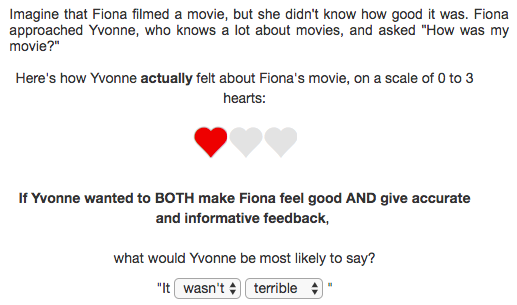
\includegraphics{fig/screenshot.png}
\caption{Example of a trial in the speaker production task.}
\end{figure}

\hypertarget{results}{%
\section{Results}\label{results}}

\begin{figure}
\centering
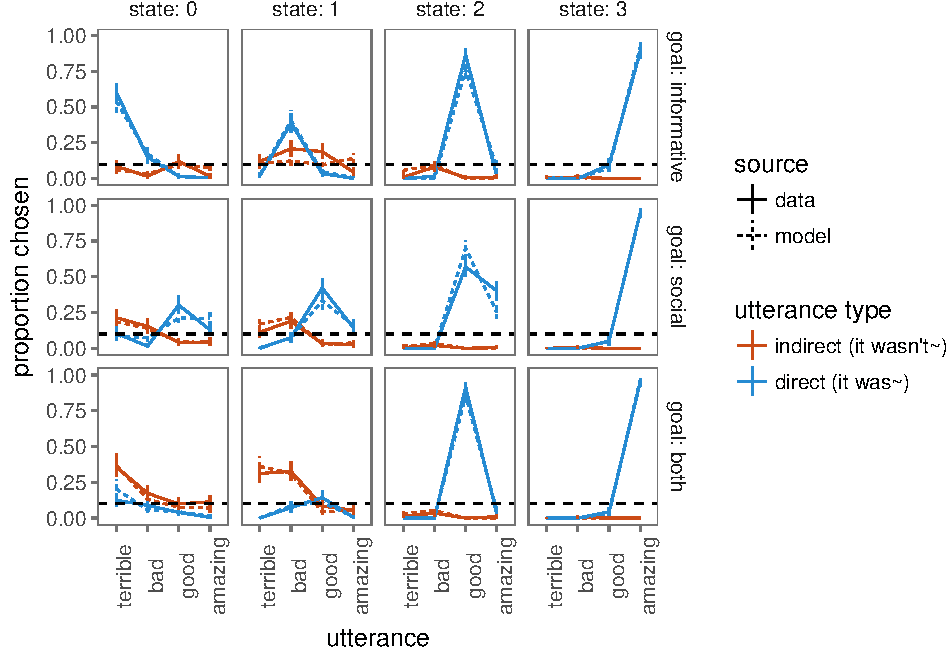
\includegraphics{politeness_files/figure-latex/utterancePrediction-1.pdf}
\caption{\label{fig:utterancePrediction}Experimental results (solid lines)
and fitted model predictions (dashed lines) for speaker production.
Proportion of utterances chosen (utterance type -- direct vs.~indirect
-- in different colors and words shown on x-axis) given the true states
(columns) and speaker goals (rows). Error bars represent 95\% confidence
intervals for the data and 95\% highest density intervals for the model.
Black dotted line represents the chance level.}
\end{figure}

\begin{figure}
\centering
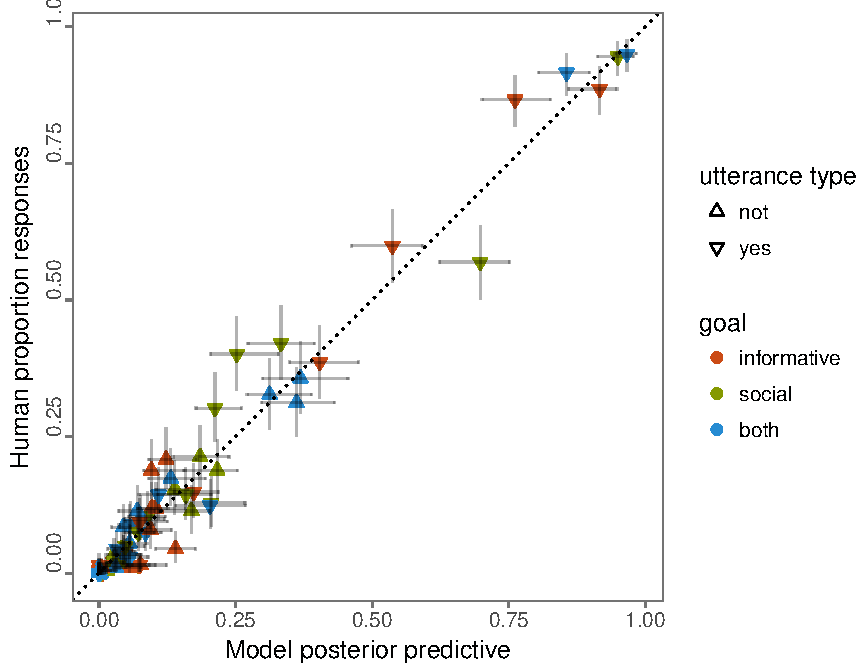
\includegraphics{politeness_files/figure-latex/varianceExplained-1.pdf}
\caption{\label{fig:varianceExplained}Full distribution of human responses
vs.~model predictions. Error bars represent 95\% confidence intervals
for the data (vertical) and 95\% highest density intervals for the model
(horizontal).}
\end{figure}

\begin{figure}
\centering
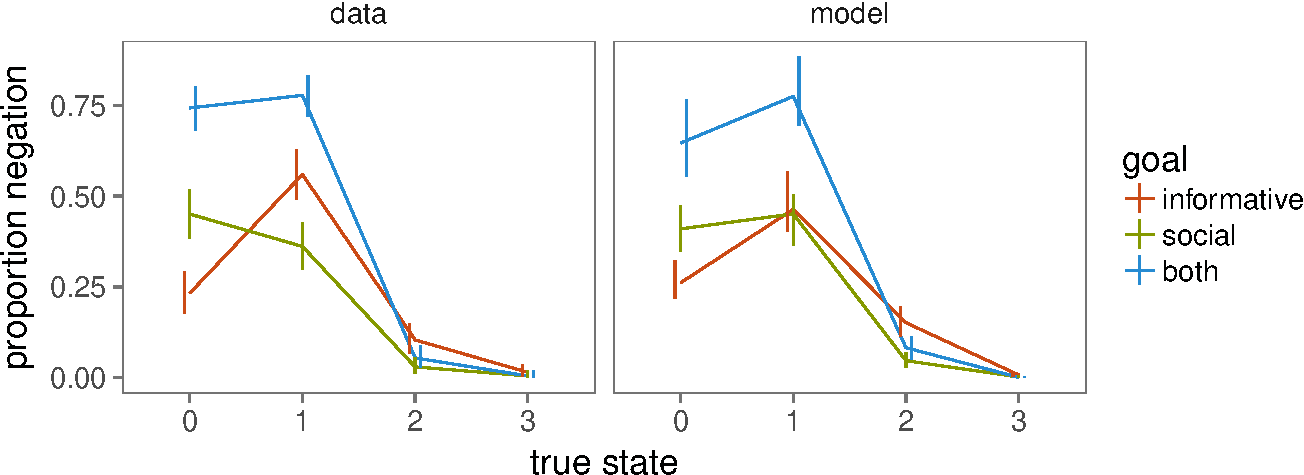
\includegraphics{politeness_files/figure-latex/negationPrediction-1.pdf}
\caption{\label{fig:negationPrediction}Experimental results (left) and
fitted model predictions (right) for average proportion of negation
produced among all utterances, given true states (x-axis) and goals
(colors).}
\end{figure}

Mean proportion of utterances chosen by participants in each true-state
\(\times\) goal condition were overall highly consistent with the our
model predictions (Figure \ref{fig:utterancePrediction}). The posterior
predictive of the model explained almost all of the variance in the
production data \(r^2\)(96) = 0.97 (Figure \ref{fig:varianceExplained}).
Consistent In line with our hypothesis, the both-goal speaker \(\times\)
bad true state (0 or 1 heart) conditions yielded the greatest proportion
of negation (\enquote{It wasn't \textasciitilde{}}; see Figure
\ref{fig:negationPrediction}).

Our work unifies previous formal models of communication and informal
theories of social uses of language. Our findings suggest that neither
epistemic nor social motives alone motivate polite speech; instead,
production of polite speech results from the conflict between these two,
combined with a self-presentational desire to \emph{look} epistemically
and socially helpful. These findings provide strong support for a
utility-theoretic framing of politeness, and suggest new directions in
understanding of pragmatic language use in social contexts.

\hypertarget{appendices}{%
\section{Appendices}\label{appendices}}

\hypertarget{literal-semantic-judgments}{%
\subsection{Literal semantic
judgments}\label{literal-semantic-judgments}}

\begin{figure}
\centering
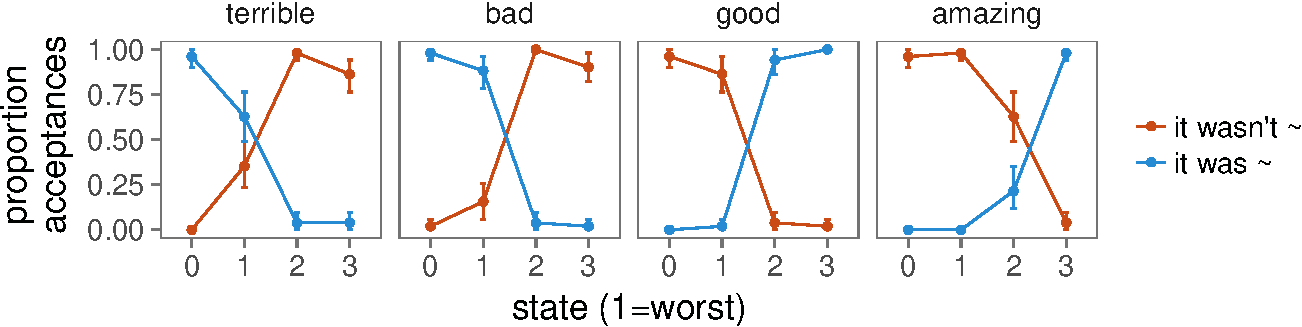
\includegraphics{politeness_files/figure-latex/litSem-1.pdf}
\caption{\label{fig:litSem}Semantic measurement results. Proportion of
acceptances of utterance types (colors) combined with target words
(facets) given the true state represented on a scale of hearts. Error
bars represent 95\% confidence intervals.}
\end{figure}

\hypertarget{inferred-parameters}{%
\subsection{Inferred parameters}\label{inferred-parameters}}

\begin{figure}
\centering
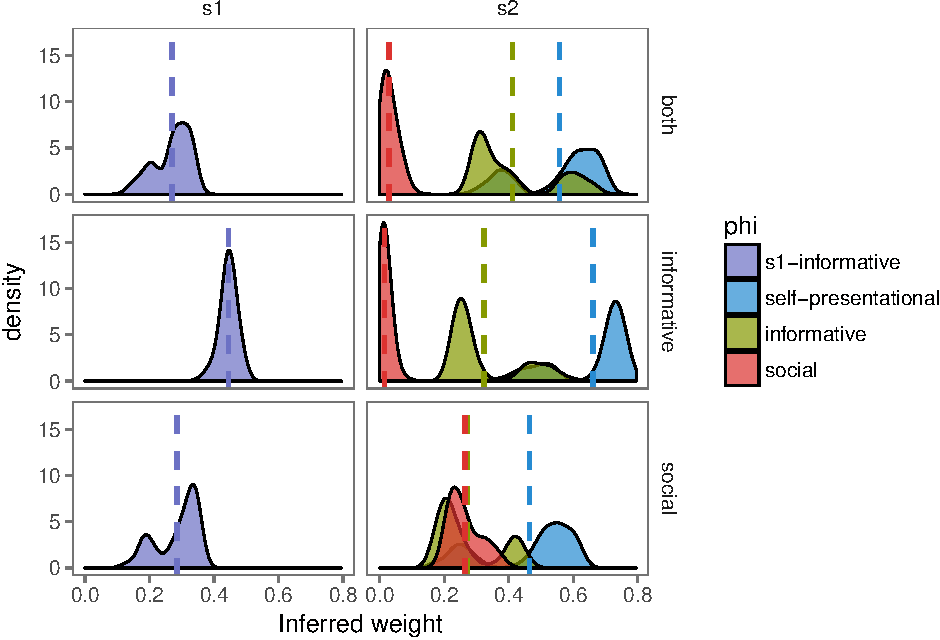
\includegraphics{politeness_files/figure-latex/goalWeights-1.pdf}
\caption{\label{fig:goalWeights}Inferred goal weights. Horizontal facets are
different experimental conditions (trying to be X). Density plots show
likely weights used in the speaker's utility function.}
\end{figure}

\begin{figure}
\centering
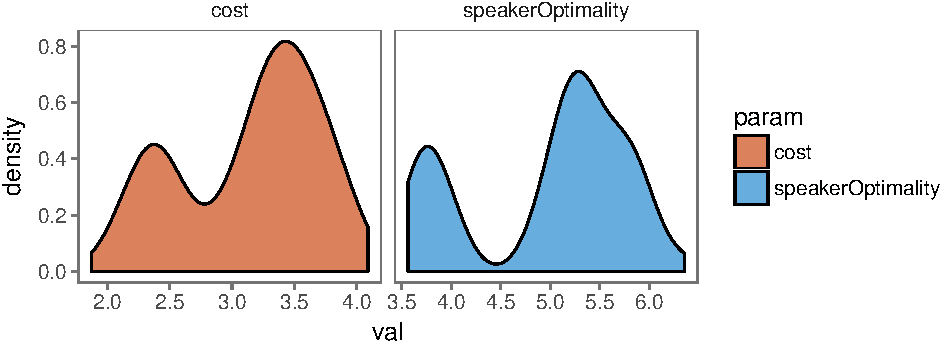
\includegraphics{politeness_files/figure-latex/params-1.pdf}
\caption{\label{fig:params}Inferred cost and speaker optimality parameters
from the main model.}
\end{figure}

\hypertarget{data-analysis-tools}{%
\subsection{Data analysis tools}\label{data-analysis-tools}}

We used R (3.4.2, R Core Team, 2017) and the R-packages \emph{bindrcpp}
(0.2, Müller, 2017), \emph{binom} (1.1.1, Dorai-Raj, 2014), \emph{coda}
(0.19.1, Plummer, Best, Cowles, \& Vines, 2006), \emph{dplyr} (0.7.4,
Wickham, Francois, Henry, \& Müller, 2017), \emph{forcats} (0.2.0,
Wickham, 2017a), \emph{ggplot2} (2.2.1, Wickham, 2009), \emph{ggthemes}
(3.4.0, Arnold, 2017), \emph{gridExtra} (2.3, Auguie, 2017),
\emph{jsonlite} (1.5, Ooms, 2014), \emph{langcog} (0.1.9001, Braginsky,
Yurovsky, \& Frank, n.d.), \emph{magrittr} (1.5, Bache \& Wickham,
2014), \emph{papaja} (0.1.0.9492, Aust \& Barth, 2017), \emph{purrr}
(0.2.4, Henry \& Wickham, 2017), \emph{readr} (1.1.1, Wickham, Hester,
\& Francois, 2017), \emph{rwebppl} (0.1.97, Braginsky, Tessler, \&
Hawkins, n.d.), \emph{stringr} (1.2.0, Wickham, 2017b), \emph{tibble}
(1.3.4, Müller \& Wickham, 2017), \emph{tidyr} (0.7.2, Wickham \& Henry,
2017), and \emph{tidyverse} (1.2.1, Wickham, 2017c) for all our
analyses.

\hypertarget{model-parameter-and-weight-comparison}{%
\subsection{Model parameter and weight
comparison}\label{model-parameter-and-weight-comparison}}

Here we compare predictions of the current model with its possible
alternatives. The current model has a triple mixture structure, with
three goals each of which is assigned a different weight: (1) goal to be
truly informative (i.e.~want to convey the true state); (2) goal to be
truly social (i.e.~want to make the listener feel good); (3)
self-presentational goal to appear certain way (as determined by
s1-phi). Alternative models involve one or two out of these three
components. Below we show that the current model best captures the
production pattern in the empirical data.

\begin{figure}
\centering
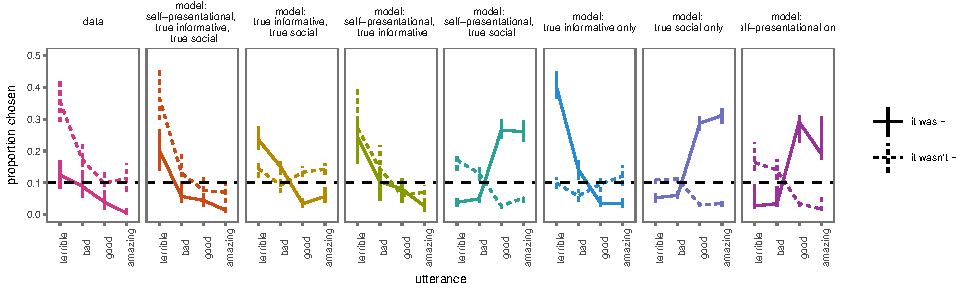
\includegraphics{politeness_files/figure-latex/utterancePredictionComp-1.pdf}
\caption{\label{fig:utterancePredictionComp}Utterances from data (leftmost)
and predictions from different model alternatives for a speaker with
both goals addressing the true state of 0 heart. Proportion of
utterances chosen (direct utterances in solid lines and indirect
utterances in dotted lines, and words shown on x-axis). Error bars
represent 95\% confidence intervals for the data and 95\% highest
density intervals for the model. Black dotted line represents the chance
level.}
\end{figure}

\begin{figure}
\centering
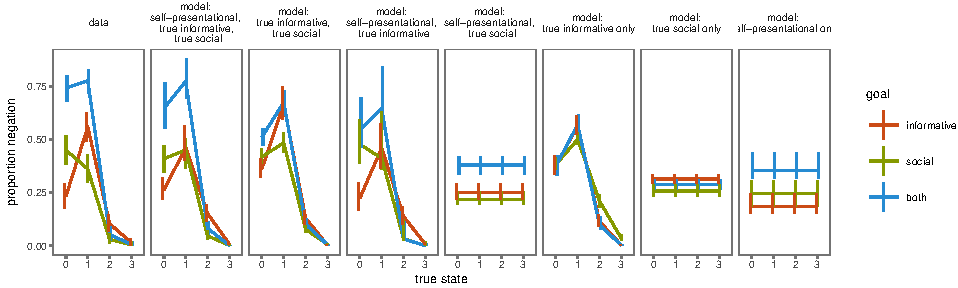
\includegraphics{politeness_files/figure-latex/negationPredictionComp-1.pdf}
\caption{\label{fig:negationPredictionComp}Experimental results (leftmost)
and predictions from different model alternatives for average proportion
of negation produced among all utterances, given true states (x-axis)
and goals (colors).}
\end{figure}

\begin{figure}
\centering
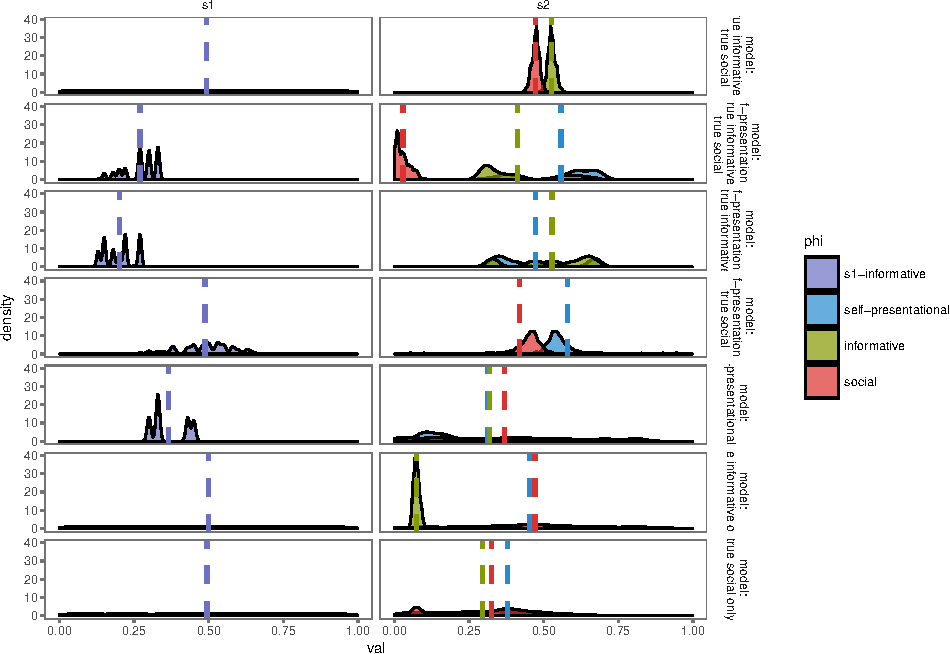
\includegraphics{politeness_files/figure-latex/goalWeightsComp-1.pdf}
\caption{\label{fig:goalWeightsComp}Inferred goal weights from different
model alternatives. Horizontal facets are different experimental
conditions (trying to be X). Density plots show likely weights used in
the speaker's utility function.}
\end{figure}

\newpage

\hypertarget{references}{%
\section{References}\label{references}}

\setlength{\parindent}{-0.5in}\setlength{\leftskip}{0.5in}

\hypertarget{refs}{}
\leavevmode\hypertarget{ref-R-ggthemes}{}%
Arnold, J. B. (2017). \emph{Ggthemes: Extra themes, scales and geoms for
'ggplot2'}. Retrieved from
\url{https://CRAN.R-project.org/package=ggthemes}

\leavevmode\hypertarget{ref-R-gridExtra}{}%
Auguie, B. (2017). \emph{GridExtra: Miscellaneous functions for "grid"
graphics}. Retrieved from
\url{https://CRAN.R-project.org/package=gridExtra}

\leavevmode\hypertarget{ref-R-papaja}{}%
Aust, F., \& Barth, M. (2017). \emph{papaja: Create APA manuscripts with
R Markdown}. Retrieved from \url{https://github.com/crsh/papaja}

\leavevmode\hypertarget{ref-R-magrittr}{}%
Bache, S. M., \& Wickham, H. (2014). \emph{Magrittr: A forward-pipe
operator for r}. Retrieved from
\url{https://CRAN.R-project.org/package=magrittr}

\leavevmode\hypertarget{ref-R-rwebppl}{}%
Braginsky, M., Tessler, M. H., \& Hawkins, R. (n.d.). \emph{Rwebppl: R
interface to webppl}. Retrieved from
\url{https://github.com/mhtess/rwebppl}

\leavevmode\hypertarget{ref-R-langcog}{}%
Braginsky, M., Yurovsky, D., \& Frank, M. (n.d.). \emph{Langcog:
Language and cognition lab things}. Retrieved from
\url{http://github.com/langcog/langcog}

\leavevmode\hypertarget{ref-brown1987}{}%
Brown, P., \& Levinson, S. C. (1987). \emph{Politeness: Some universals
in language usage} (Vol. 4). Cambridge university press.

\leavevmode\hypertarget{ref-R-binom}{}%
Dorai-Raj, S. (2014). \emph{Binom: Binomial confidence intervals for
several parameterizations}. Retrieved from
\url{https://CRAN.R-project.org/package=binom}

\leavevmode\hypertarget{ref-goodman2013}{}%
Goodman, N. D., \& Stuhlmüller, A. (2013). Knowledge and implicature:
Modeling language understanding as social cognition. \emph{Topics in
Cognitive Science}, \emph{5}(1), 173--184.

\leavevmode\hypertarget{ref-grice1975}{}%
Grice, H. P. (1975). Logic and conversation. In P. Cole \& J. L. Morgan
(Eds.), \emph{Syntax and semantics} (Vol. 3, pp. 41--58). Academic
Press.

\leavevmode\hypertarget{ref-R-purrr}{}%
Henry, L., \& Wickham, H. (2017). \emph{Purrr: Functional programming
tools}. Retrieved from \url{https://CRAN.R-project.org/package=purrr}

\leavevmode\hypertarget{ref-R-bindrcpp}{}%
Müller, K. (2017). \emph{Bindrcpp: An 'rcpp' interface to active
bindings}. Retrieved from
\url{https://CRAN.R-project.org/package=bindrcpp}

\leavevmode\hypertarget{ref-R-tibble}{}%
Müller, K., \& Wickham, H. (2017). \emph{Tibble: Simple data frames}.
Retrieved from \url{https://CRAN.R-project.org/package=tibble}

\leavevmode\hypertarget{ref-R-jsonlite}{}%
Ooms, J. (2014). The jsonlite package: A practical and consistent
mapping between json data and r objects. \emph{arXiv:1403.2805
{[}stat.CO{]}}. Retrieved from \url{https://arxiv.org/abs/1403.2805}

\leavevmode\hypertarget{ref-R-coda}{}%
Plummer, M., Best, N., Cowles, K., \& Vines, K. (2006). CODA:
Convergence diagnosis and output analysis for mcmc. \emph{R News},
\emph{6}(1), 7--11. Retrieved from
\url{https://journal.r-project.org/archive/}

\leavevmode\hypertarget{ref-R-base}{}%
R Core Team. (2017). \emph{R: A language and environment for statistical
computing}. Vienna, Austria: R Foundation for Statistical Computing.
Retrieved from \url{https://www.R-project.org/}

\leavevmode\hypertarget{ref-R-ggplot2}{}%
Wickham, H. (2009). \emph{Ggplot2: Elegant graphics for data analysis}.
Springer-Verlag New York. Retrieved from \url{http://ggplot2.org}

\leavevmode\hypertarget{ref-R-forcats}{}%
Wickham, H. (2017a). \emph{Forcats: Tools for working with categorical
variables (factors)}. Retrieved from
\url{https://CRAN.R-project.org/package=forcats}

\leavevmode\hypertarget{ref-R-stringr}{}%
Wickham, H. (2017b). \emph{Stringr: Simple, consistent wrappers for
common string operations}. Retrieved from
\url{https://CRAN.R-project.org/package=stringr}

\leavevmode\hypertarget{ref-R-tidyverse}{}%
Wickham, H. (2017c). \emph{Tidyverse: Easily install and load the
'tidyverse'}. Retrieved from
\url{https://CRAN.R-project.org/package=tidyverse}

\leavevmode\hypertarget{ref-R-tidyr}{}%
Wickham, H., \& Henry, L. (2017). \emph{Tidyr: Easily tidy data with
'spread()' and 'gather()' functions}. Retrieved from
\url{https://CRAN.R-project.org/package=tidyr}

\leavevmode\hypertarget{ref-R-dplyr}{}%
Wickham, H., Francois, R., Henry, L., \& Müller, K. (2017). \emph{Dplyr:
A grammar of data manipulation}. Retrieved from
\url{https://CRAN.R-project.org/package=dplyr}

\leavevmode\hypertarget{ref-R-readr}{}%
Wickham, H., Hester, J., \& Francois, R. (2017). \emph{Readr: Read
rectangular text data}. Retrieved from
\url{https://CRAN.R-project.org/package=readr}






\end{document}
